%
% Registrierung astronomischer Bilder
%
% (c) 2013 Prof Dr Andreas Mueller, Hochschule Rapperswil
%
\subsection{Registrierung astronomischer Bilder}
In vielen wissenschaftlichen Anwendungen ist es notwendig, Bilder auf
ein bestimmtes Raster auszurichten. So ist es zum Beispiel möglich,
aus einer Serie leicht verschobener Bilder der gleichen Szene durch
Überlagerung ein Bild höherer Auflösung zu gewinnen.

Die Technik ist auch verbreitet in der Astrophotographie. Am Sternenhimmel
findet man nahe beieinander Objekte extrem unterschiedlicher Helligkeit.
Der Planet Saturn strahlt etwa $10^{10}$ mal mehr Licht ab, als sein
4km grosser Mond Fenrir.
Auch hochwertige CCD-Kameras für Astrophotographie verwenden jedoch nur
A/D-Wandler mit 16bit, erlauben also nur ein maximales
Helligkeitsverhältnis von $65535 : 1$ ohne Sättigung.
Um Fenrir und Saturn auf dem gleichen Bild sichtbar zu machen, müsste
ein 34bit-A/D-Wandler verwendet werden, und der CCD-Chip und
Eingangsverstärker müssten entsprechend rauscharm sein.

\begin{figure}
\begin{center}
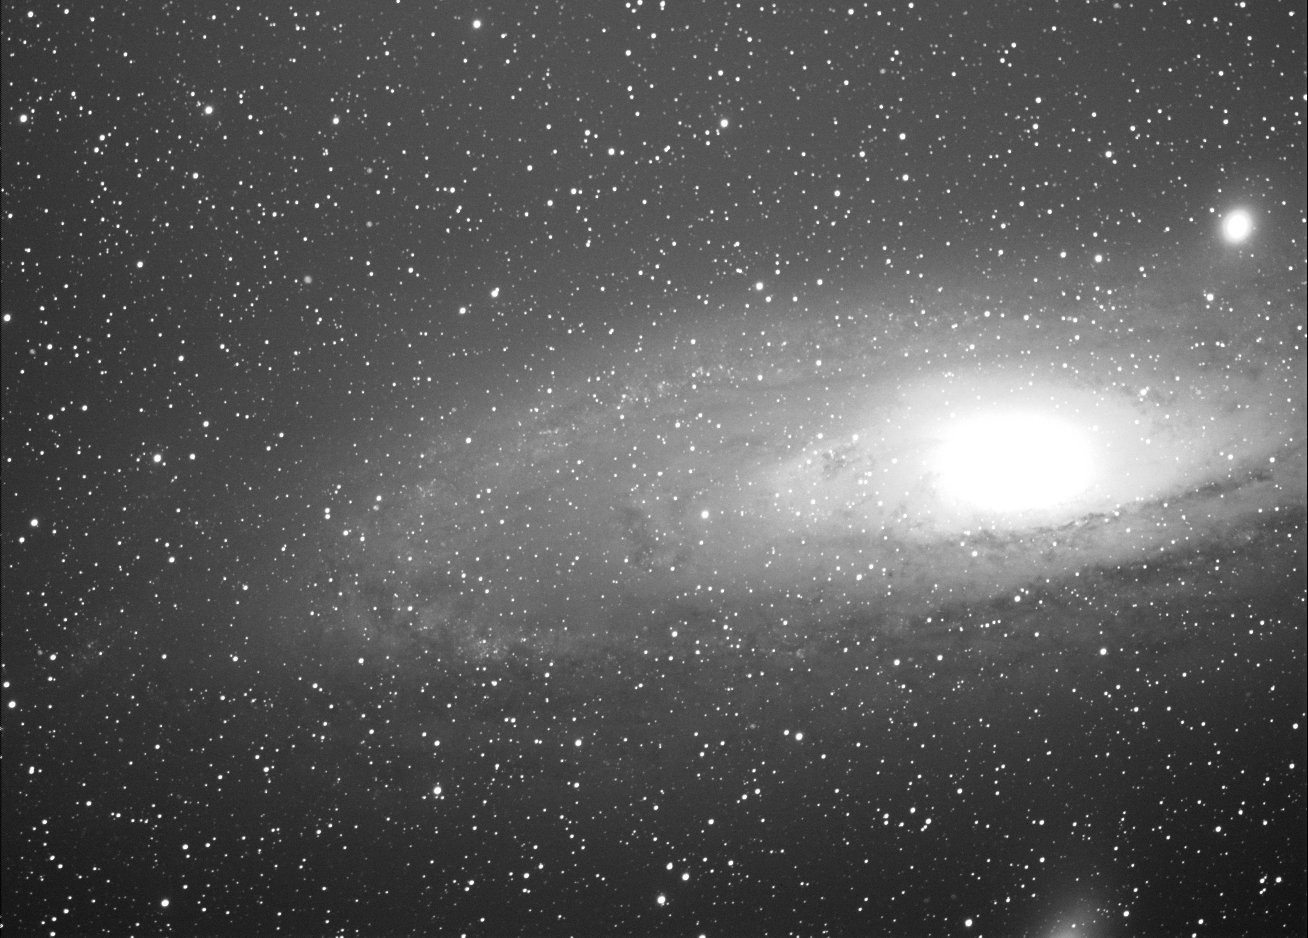
\includegraphics[width=\hsize]{graphics/andromeda-gimped.jpg}
\end{center}
\caption{Aus 10 Aufnahmen zusammengesetzte Aufnahme der Andromeda Galaxie
M31.\label{andromeda-image}}
\end{figure}

Astrophotographen erstellen daher mehrere Bilder des gleichen Objekts
mit vergleichsweise kurzer Belichtungszeit von wenigen Minuten, und
addieren diese später auf dem Computer. Dazu müssen die Bilder
exakt zur Deckung gebracht werden.
Ein besonders spektakuläres Beispiel dieser Technik ist das Hubble
Deep Field (HDF), welches 342 Einzelaufnahmen von Total
etwa 140.8 Stunden Belichtungszeit kombiniert.
Es zeigt etwa 3000 Galaxien, aber nur etwa 20 Sterne aus unserer eigenen
Galaxie. 

Wegen der geringen Lichtmenge verwenden Astronomen Teleskope mit
grossen Spiegeln, die viel Licht sammeln können. Trotzdem sind lange
Belichtungszeiten nötig, um ein verwertbares Signal zu erhalten,
mehrere Stunden Belichtung sind nicht ungewöhnlich.
Damit steigt jedoch auch das Rauschsignal des CCD-Chips an, weshalb
CCD-Kameras gekühlt werden müssen, entweder mit flüssigem Stickstoff
oder sogar flüssigem Helium, oder für kleine Observatorien thermoelektrisch
mit Hilfe von Peltier Elementen.
Die damit erreichbaren Temperaturen sind jedoch wesentlich höher,
ca.~50 Grad Celsius unter der Umgebungstemperatur.

Permanent aufgestellte professionelle Teleskope arbeiten genau
genug, dass sich die Bilder durch eine kleine Translation zur
Deckung bringen lassen.
Diese Translation kann mit Hilfe von Fourier-Transformation sehr
schnell gefunden werden.
Mobile Teleskope haben aber immer einen verbleibenden Aufstellungsfehler,
der zu einer Rotation des Bildes während der Beobachtungszeit führen.
Grossteleskop wie das Very Large Teleskop auf dem Cerro Paranal in
Chile sind sie schwer, dass sie nur mit einer sogenannten azimutalen
Montierung aufgestellt werden können, hier ist die Bildfelddrehung
unvermeidlich.
Natürlich kann auch diese Drehung mechanisch mit einem sogenannten
Rotator kompensiert werden, dieser beträchtliche Aufwand lässt sich
für kleine Teleskope jedoch nicht rechtfertigen.

Alle diese Faktoren limitiert die Belichtungszeit auf wenige Minuten.
Solange die Rotation in den
Randbereichen eines Bildes kleiner als ein Pixel bleibt, stört
sie nicht.
Ein Bild mit langer Belichtungszeit lässt sich also nur dann erstellen,
wenn man viele Bilder mit kurzer Belichtungszeit aufaddiert.

Ausserdem sind astronomische Kameras monochrom, die Farben entstehen
dadurch, dass das gleiche Objekt durch verschiedene Farbfilter photographiert
wird. Auch diese Bilder müssen für ein farbiges Bild zur Deckung
gebracht werden, und auch in diesem Fall sind ausser Verschiebungen
auch Drehungen möglich. 

Eine weitere mögliche Anwendung ist die Kombination von Bildern von
verschiedenen Teleskopen in ein synthetisches Bild, welches zum Beispiel
gleichzeitig die Strahlung im sichtbaren Bereich und im Röntgen-Bereich
zeigt, aufgenommen von einem Teleskop im Erdorbit.

Es ist also folgendes Problem zu lösen:

\begin{aufgabe}
Ein Bild mit Pixeln in einem
$x$-$y$-Koordinatensystem muss so deformiert werden, dass es möglichst
gut auf ein anderes Bild passt. Dabei darf man annehmen, dass es eine
schnelle und genaue Methode gibt, kleine Translationen zwischen Bildern 
zu ermitteln.
\end{aufgabe}

\subsubsection{Modell}
Wir müssen also Pixel vom $x$-$y$-Koordinatensystem in das Koordinatensystem
des zweiten Bildes. Wir gehen davon aus, dass Geraden im einen Bild
auch Geraden im anderen Bild sind, in erster Näherung ist dies sicher
zulässig\footnote{Insbesondere bei Weitwinkelkameras trifft diese Annahme
nicht mehr zu, da wird das Bild nichtlinear verzerrt. Der hier vorgestellte
Lösungsansatz lässt sich jedoch auf diesen Fall erweitern.}.
Die Koordinatentransformation ist also linear, wir setzen sie an in der
Form
\begin{equation}
\begin{linsys}{4}
x'&=&a_{11} x&+&a_{12}y&+&t_1\\
y'&=&a_{21} x&+&a_{22}y&+&t_2\\
\end{linsys}
\label{registration:model}
\end{equation}
oder in Matrizenform
\[
\begin{pmatrix}
x'\\
y'
\end{pmatrix}
=A\begin{pmatrix}x\\y\end{pmatrix}+t
\]
Die Aufgabe ist gelöst, sobald die Matrix $A$ und der Vektor $t$ bestimmt
sind, also insgesamt 6 Unbekannte.

\subsubsection{Lösung}
In einem kleinen Gebiet des Bildes ist die Transformation
(\ref{registration:model}) nicht von einer Translation zu unterscheiden.
Um die Drehung oder Streckung zu sehen, die in der Matrix $A$ drin stecken
kann, muss ein grösseres Gebiet des Bildes betrachtet werden. 

Um die Transformation (\ref{registration:model}) zu ermitteln, kann man
also versuchen in einzelnen Gebieten des Bildes die dort vorherrschende
Translation zu finden. Dann sucht man die Transformation, welche die
Translationen in den einzelnen Bildteilen am besten wiedergibt.

Man zerlegt dazu die Bilder in einzelne Kacheln von $128 \times 128$ Pixeln.
Die Kachel mit der Nummer $i$ hat ihr Zentrum im Punkt $(x_i,y_i)$.
Die entsprechende Kachel im zweiten Bild ist gegenüber der ersten
um einen Vektor $\delta_i=(\delta_{i,x},\delta_{i,y})$ verschoben.
Gäbe es eine exakte Lösung, müssten die Gleichungen
\[
\begin{linsys}{7}
x_i+\delta_{i,x}&=&x_ia_{11}&+&y_ia_{12}&+&t_1& &         & &         & &    \\
y_i+\delta_{i,y}&=&         & &         & &   & &x_ia_{21}&+&y_ia_{22}&+& t_2\\
\end{linsys}
\]
für die sechs Unbekannten $a_{jk}$ und $t_j$ exakt erfüllt sein.
Bei $n$ Kacheln sind dies $2n$ Ungleichungen, das Gleichungssystem ist
also überbestimmt.
Es lässt sich mit der Methode von Abschnitt \ref{section:ueberbestimmt}
effizient lösen.

Abbildung~\ref{andromeda-image} zeigt das Resultat der Anwendung dieses
Algorithmus auf 10 Bilder mit je 2 Minuten Belichtungszeit.
Der CCD-Chip der verwendeten Kamera misst $3900\times 2616$ Pixel, darin
finden $n=600$ Kacheln $128\times 128$ Platz.
Zur Bestimmung der Transformation wurde also für jedes Teilbild
ein überbestimmtes Gleichungssystem mit 1200 Gleichung für die
sechs Unbekannten gelöst. Auf einem modernen Computer dauert dies
nur Sekundenbruchteile, die nachfolgende Anwendung der Transformation
auf die Bilder ist bei weitem zeitaufwendiger.

